\documentclass[../main.tex]{subfiles}


\begin{document}

\onehalfspacing

%-------------------------------------------------------------------------
%----------------------------------REDES----------------------------------
%-------------------------------------------------------------------------


En este capítulo, se mostrarán los fundamentos teóricos utilizados en este trabajo. Se comienza con teoría de redes y termina con una síntesis de la entropía de Shannon. 

\section{Teoría de Redes.}
%Es un breve resumen sobre redes (inlcuir a Euler, Moreno, Milgram, Strogatz, Babarbasi)

% A continuación, se presentará un contexto histórico del desarrollo de la teoría de redes. 


El problema de los puentes de Königsberg resulta ser una de las primeras motivaciones en la teoría de gráficas. La  ciudad de Königsberg fue fundada por los caballeros teutónicos en el año 1255 y, debido a su asentamiento sobre el río Pregolia, se convirtió en un importante centro de intercambio. Por ello, la ciudad fue dividida en cuatro regiones conectadas por siete puentes (ver figura \ref{fig:marcoteorico_konigsberg}).



\begin{figure}[h!]
    \centering
    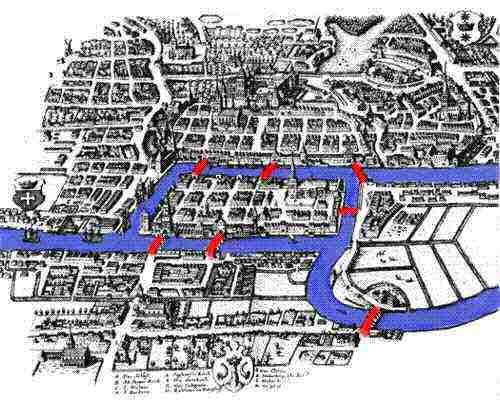
\includegraphics[scale = 0.5]{images/marcoteorico_konigsberg.jpg}
    \caption{Una vista de Königsberg mostrando en rojo los siete puentes sobre el río Pregolia.  }
    \label{fig:marcoteorico_konigsberg}
\end{figure}


El problema de los siete puentes de Königsberg que conectan las cuatros regiones intenta resolver la siguiente pregunta:  ¿es posible dar un paseo por todas las regiones,  comenzando desde cualquiera de estas regiones, pasando por todos los puentes una sola vez y regresando al mismo punto de partida? 

Fue hasta el año 1736 cuando se hace público el artículo de Leonhard Euler dando una solución particular y general a este problema. Lo más esencial de este texto de 21 párrafos es la simplicidad de la solución. Euler propone enfocarnos en las conexiones generadas por los puentes; explícitamente, identificar a cada segmento de tierra con una letra mayúscula y cada puente con una letra minúscula (ver figura \ref{fig:marcoteorico_abstracteuler}).   De la representación de Euler, se obtuvieron  resultados generales a través de varios experimentos. 

Es curioso mencionar que debido a la sencillez del planteamiento del problema de los puentes, Euler no creía necesaria la intervención de una visión matemática [\cite{thetrueaboutkonigsberg}], sin embargo, la abstracción que realizó dio inicio una rama más de la Matemática: Teoría de Gráficas. 

%  No coincide con las fechas
% Este artículo motivó el enfoque de los problemas en una abstracción de objetos y sus relaciones. Con ello, el inicio de una rama más de la Matemática: Teoría de Gráficas.  



\begin{figure}[h!]
    \centering
    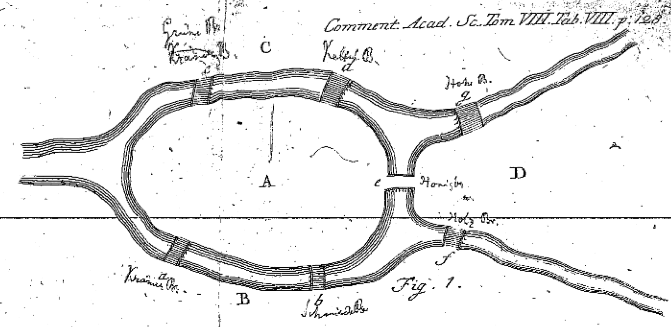
\includegraphics[scale = 0.5]{images/marcoteorico_abstract.png}
    \caption{Esbozo original de Euler sobre el problema de los puentes de Königsberg.}
    \label{fig:marcoteorico_abstracteuler}
\end{figure}


%Dejemos pendiente Jacobo Levy Moreno
%Some ideas: 
%-Breve descripción de socioMETRÍA. -c
%Metemos a Jacabo con alguna aportación importante. -c

%  Quien tambié realizó una bas


% Idea de B

% Tiempo después, en el siglo XIX, JLM, influenciado por diversas culturas y diferencias sociales, también realizó una abstracción considerando las relaciones humanas. 

%Checar la redacción del video de hoy 25/Mayo


                %Intuitiva
Una abstracción sencilla para un pensamiento actual es extrapolar los puentes hacia las relaciones humanas, algo innovador para el pensamiento del siglo XIX. Jacobo Levy Moreno, influenciado por diversas culturas y diferencias sociales, consideró la afinidad y preferencia de la gente por relacionarse ante distintas adversidades [\cite{moreno_intro}]. Esta observación dio origen a la sociometría que fue impulsada por los sociogramas: representaciones gráficas de relaciones sociales.


%Standley Milgran; principios del Mundo pequeño. 
%En continucación a estudio social, 
% Milgra and Stay, continuó trabajando con el comportamiento social. 
%
% \todo{El conector 'Al seguir la linea' no creo que sea conveniente}
Al seguir la línea del análisis del comportamiento social, en 1967,  Stanley Milgram introdujo una pregunta relacionada con situaciones cotidianas, asociada al fenómeno de \textit{mundo pequeño}: el efecto que cualesquiera dos personas en el mundo están a pocas personas de conocerse. La pregunta que planteaba era sencilla: ¿cuántas conexiones entre dos personas son necesarias para que estas se conocieran? El problema y solución considerarían la estructura matemática de la sociedad. La parte experimental de este proceso concluyó que la cantidad de personas intermedias es apenas un poco más de cinco personas [\cite{milgram1967small}]. 


No fue sino hasta finales del siglo XX que comenzó una formalización de las observaciones antes vistas. En 1998, Duncan Watts  y  Steven Strogatz, a través de un modelo que itera probabilísticamente las aristas de una red regular, encontraron una dinámica interesante en función de la estructura topológica de la red [\cite{Watts1998}]. En específico, se mostró un umbral donde la red tiene un coeficiente de agrupamiento alto pero con una corta distancia media entre los nodos.  Si bien esta conclusión de la propiedad de mundo pequeño nunca fue definitiva, motivó una formalización e investigación del fenómeno; aunque, muchas investigaciones son en función de lo mostrado por Watts y Strogatz [\cite{Telesford2011}].  

% indujo diversas incertidumbres y otras formalizaciones de la misma


% A partir de la motivación
Poco después del trabajo de Watts y Strogatz, la investigación de Barabási dentro del mundo de los sistemas complejos fomentó aun más la investigación en redes. En 1999, poco después de la publicación de Watts y Strogatz, Albert-László Barabási y Réka Albert analizaron la red de citas de páginas de Internet. El aspecto más relevante del trabajo de citas de portales de Internet era inducir una nueva dinámica en redes desde un paradigma distinto al aleatorio: Las \textit{redes de libre escala} [\cite{Barabasi1999}]. Este tipo de red presenta una propiedad interesante en su distribución de grado, pues se distribuye como una ley de potencia; de manera formal, si $f(x)$ es la distribución de grado, entonces $f$ es ley de potencia si $f(x) \sim x^{-\alpha} $, con $\alpha > 0$. Esta caracterización de la distribución de grado induce a que la red en cuestión contenga \textit{hubs} (nodos con un grado muy alto).  Esto último consecuencia de dos propiedades relevantes: el continuo nacimiento de nuevos enlaces y la preferencia de relacionarse a un nodo en particular [\cite{Barabsi2005}].  


\begin{figure}[h!]
    \centering
    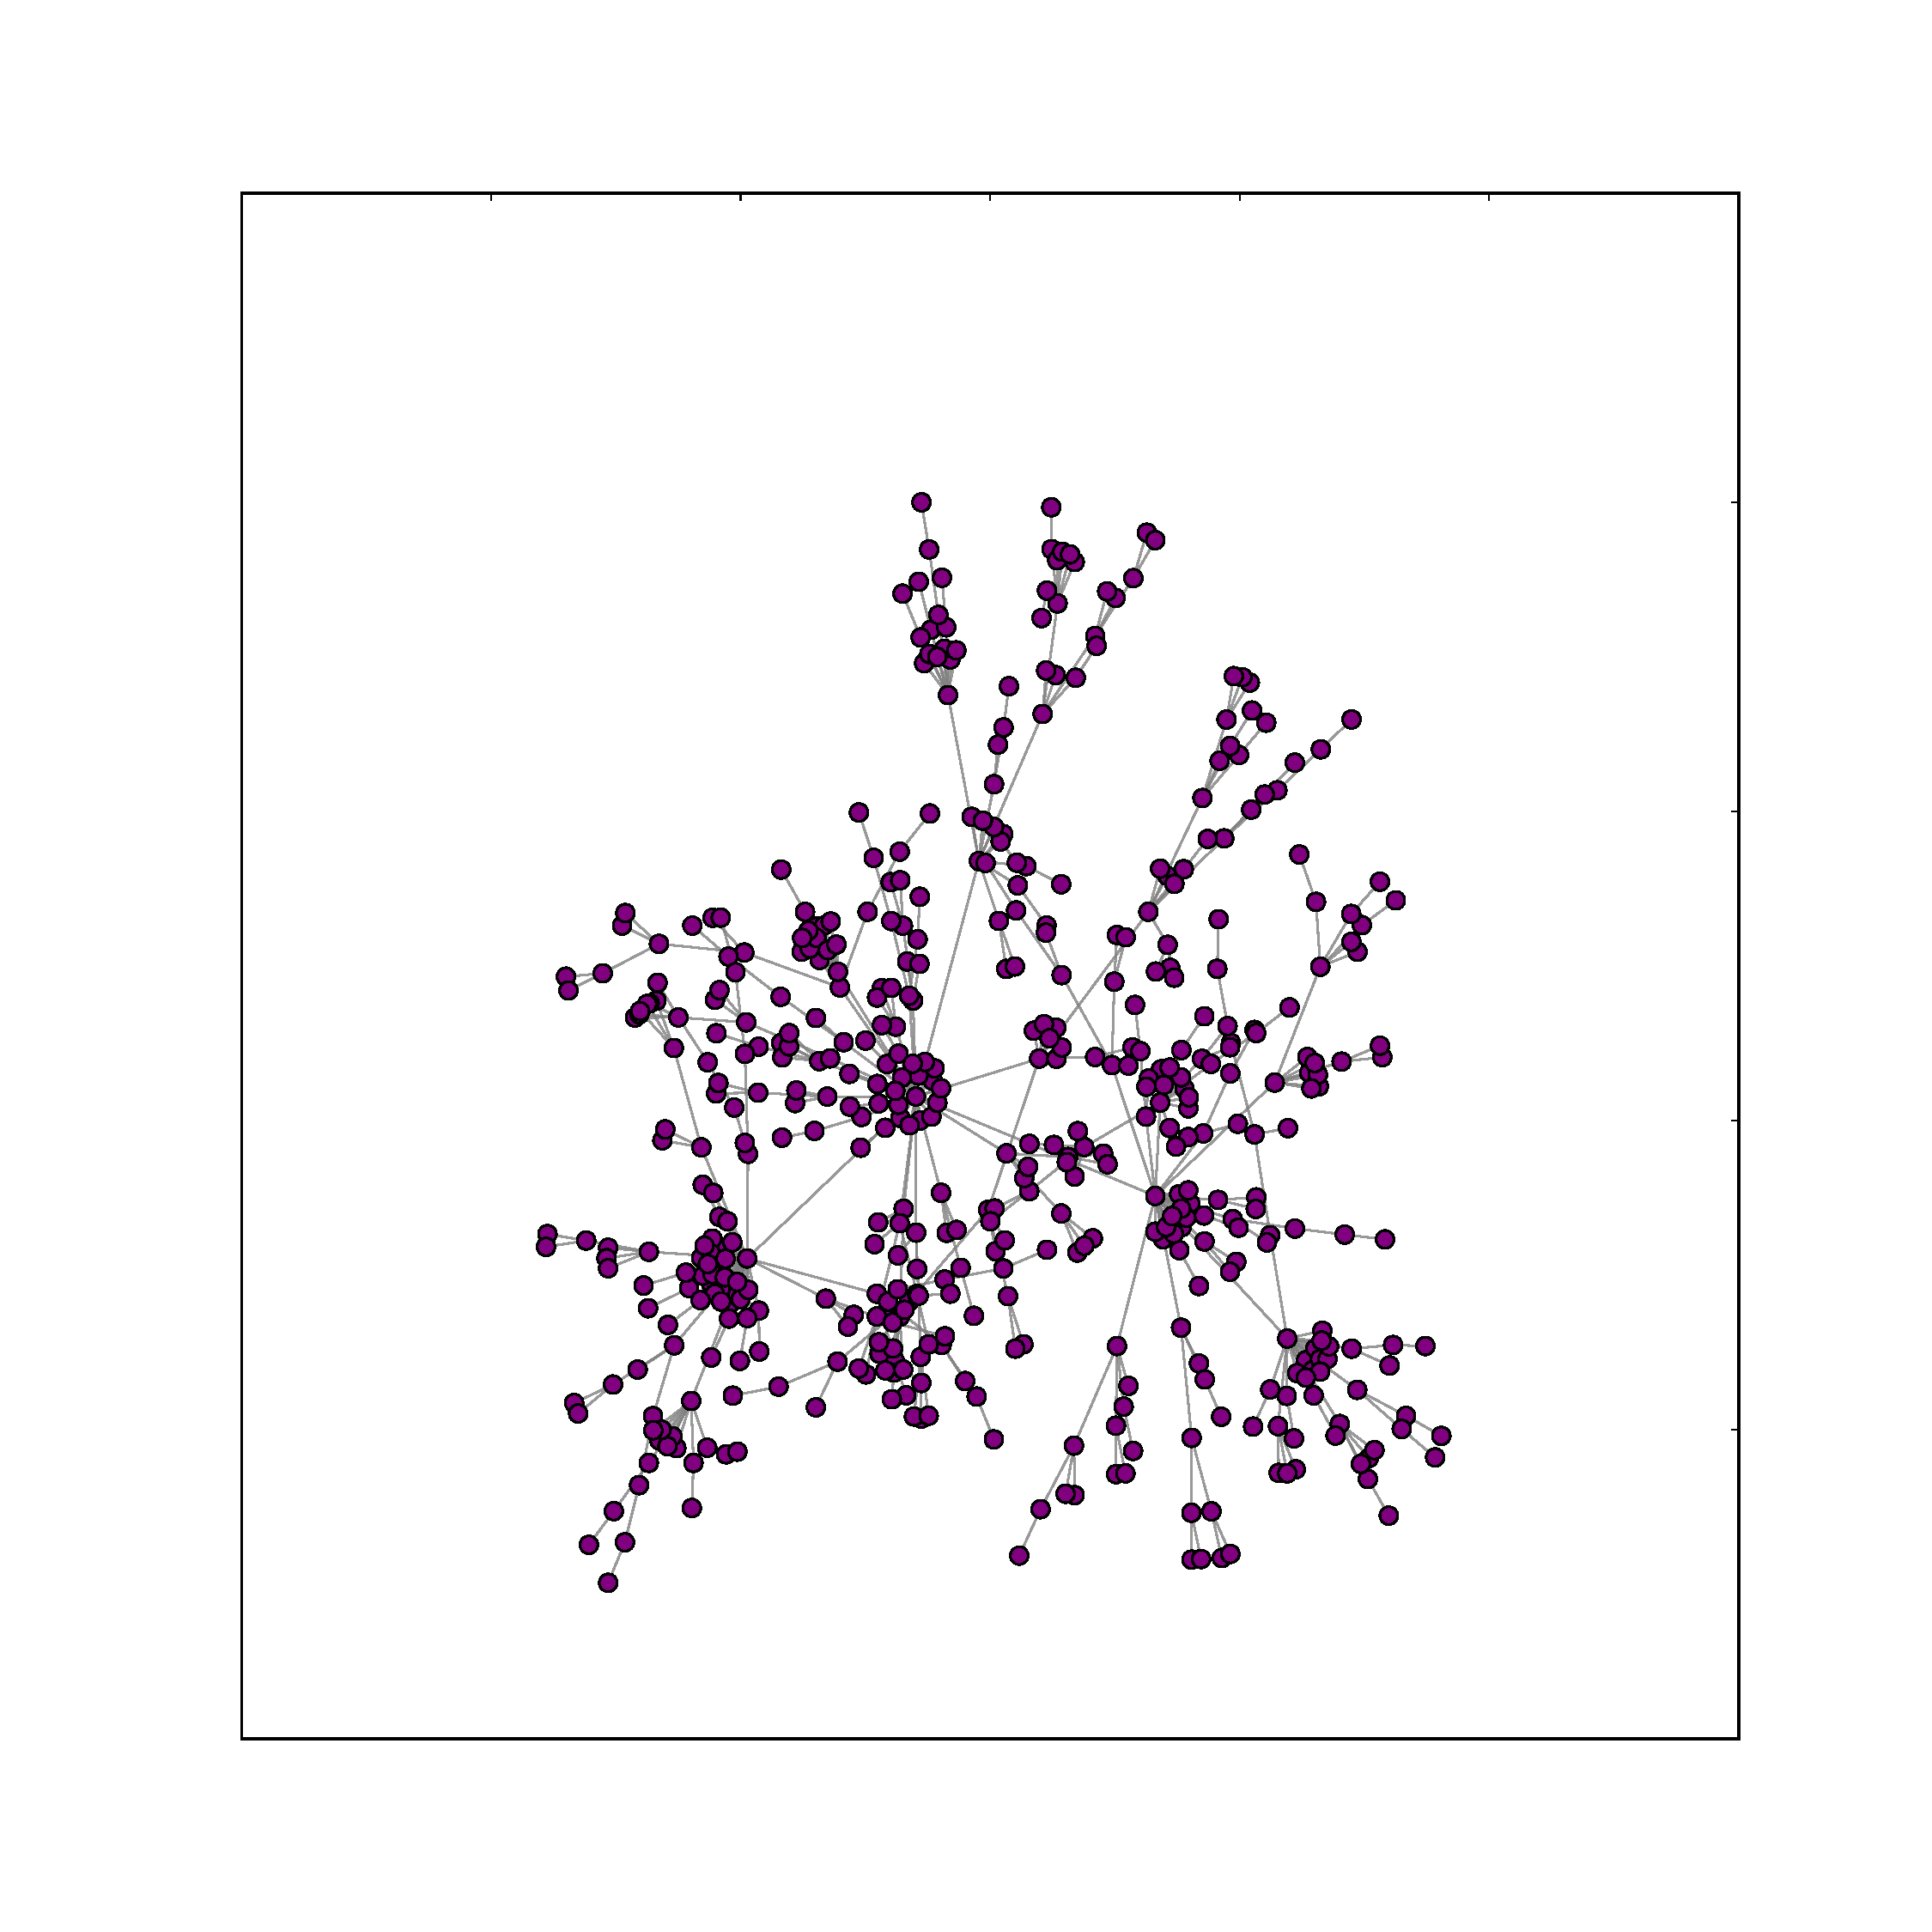
\includegraphics[scale = 0.35]{images/marcoteorico_barabasi.pdf}
    \caption{Ejemplo de una red de libre escala. Fuente: Elaboración propia.}
    \label{fig:marcoteorico_scale_free}
\end{figure}

%Como lo mencionan Strogatz 


% \begin{figure}
% \centering
% \begin{minipage}{.5\textwidth}
%   \centering
%   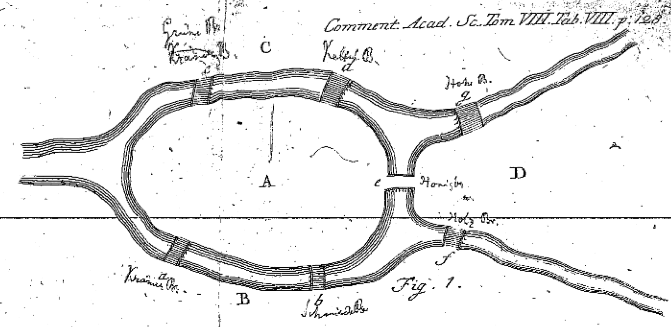
\includegraphics[width=.4\linewidth]{images/marcoteorico_abstract.png}
%   \captionof{figure}{A figure}
%   \label{fig:test1}
% \end{minipage}%
% \begin{minipage}{.5\textwidth}
%   \centering
%   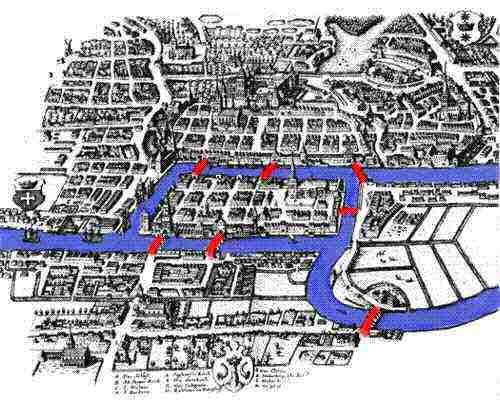
\includegraphics[width=.4\linewidth]{images/marcoteorico_konigsberg.jpg}
%   \captionof{figure}{Another figure}
%   \label{fig:test2}
% \end{minipage}
% \end{figure}

\newpage
\subsection{Definiciones de Teoría de Redes}

%Definimos una red en general.
% En esta sección se presentarán las definiciones formales de una red.

 Una \textit{gráfica} es una estructura matemática compuesta de dos partes: los objetos y las relaciones que se tienen entre ellos. Es decir, una red es una colección de puntos unidos de dos en dos por líneas [\cite{newman2018networks}]. Así, una \textit{red} es una gráfica con alguna interpretación. Los objetos y las relaciones son nombrados de diferentes maneras dependiendo del contexto y la interpretación de la red del sistema (véase la tabla \ref{tab:marcoteorico_tabladenodosenlaces} para algunos ejemplos y su interpretación, para más información ver [\cite{barabasi2013network}] ). 

En general, los objetos pueden ser distinguidos como \textit{nodos} y las relaciones como \textit{aristas}. 
% En este trabajo, el \textit{conjunto de nodos} es denotado por la letra $V$ y el \textit{conjunto de aristas} por la letra $E$.  

\newpage

\begin{table}[h!]
    \centering
    \caption{Comparativo de redes respecto a los nombres de los nodos y aristas. (Fuente: [\cite{barabasi2013network}] )}
    \begin{tabular}{c|c|c|c}
        \textit{\textbf{Red}} & \textbf{\textit{Nodos}} & \textbf{\textit{Enlaces}}  & \textbf{\textit{Tipo de red}}\\
        \hline
        Internet & Routers & Conexión de internet & No dirigida \\
        World Wide Web & Páginas web & Enlaces & Dirigida \\
        Red eléctrica & Centrales eléctricas  & Cables & No dirigida \\
        Red de actores & Actores  & Coactuación & No dirigida \\
    \end{tabular}
    
    \label{tab:marcoteorico_tabladenodosenlaces}
\end{table}

De manera formal, una red es el par ordenado de dos conjuntos

\begin{equation}
    \label{eq:marcoteorico_networkdefinition}
    G = (V,E),
\end{equation}
donde $V$ y $E$  son el conjunto de nodos y aristas, respectivamente.


Una propiedad que podría definir el tipo de red es si la arista tiene o no dirección. Una \textit{arista dirigida} es aquella donde el orden de los nodos es importante; de forma contraria, una \textit{arista no dirigida} es aquella donde el orden de los nodos es irrelevante. 

%Una propiedad que podría definir el tipo de red es si la arista tiene o no dirección. 
% La propiedad del tipo de arista podría definir el tipo de red
Lo anterior conlleva a que una \textit{red dirigida} tiene todas sus aristas dirigidas. De forma contraria, una \textit{red no dirigida} es aquella donde todas sus aristas son no dirigidas.  

%

Es decir, una red dirigida cumple con

\begin{equation*}
    (a,b) \neq (b,a), \quad \text{con } a,b \in V,
\end{equation*}

Y, por otra parte, una red no dirigida cumple con

\begin{equation*}
    (a,b) = (b,a), \quad \text{con } a,b \in V,
\end{equation*}



% Una relación entre los nodos y las aristas es el conteo de ocurrencias de un nodo en las aristas; este concepto es denominado grado de un nodo.
El \textit{grado de un nodo} es el número de aristas que tiene el nodo con los demás nodos [\cite{barabasi2013network}]. Este valor es denotado por $k_v$ donde $v$ es un nodo. 
% Es decir, desde una interpretación social,  este número representa la cantidad de interacciones que tiene un nodo con los demás nodos.

% En función del tipo de red, el grado de un nodo puede especificarse por el tipo de red. 

Para una red dirigida, el grado de un nodo se extiende a dos casos: grado interior y grado exterior.  
El \textit{grado interior} de un nodo es el número de aristas donde el nodo en cuestión es el nodo final. El \textit{grado exterior} de un nodo es el número de aristas donde el nodo en cuestión es el nodo inicial. De forma explícita, consideremos una arista,

%  El \textit{nodo inicial} y el \textit{nodo final} son la referencia al lugar en donde está colocado el nodo en la arista.

\begin{align*}
    (s,t) \in E, &\quad \text{donde } s,t \in V, \\
    s &\quad \text{ es el nodo inicial,} \\
    t &\quad \text{ es el nodo final.} \\
\end{align*}

El grado exterior de un nodo $v$ es denotado por $k^{out}_v$ y el grado interior de un nodo es denotado por $k^{in}_v$.  

Así, de manera formal, el grado exterior e interior de un nodo se definen como:  

\begin{align*}
k^{out}_v &= \left|\left\{ \quad (x,v) \in E \quad | \quad x \in V \quad  \right\}\right|,  \\
k^{in}_v &= \left|\left\{ \quad (v,x) \in E \quad | \quad x \in V \quad  \right\}\right|,  \\
\end{align*}

donde $|A|$ representa la cardinalidad del conjunto $A$. 

Cabe mencionar que para el caso de una red no dirigida, donde el orden las aristas no es relevante, el grado de un nodo es igual a cualquiera de los casos anteriores, es decir, 


\begin{align*}
    k_v = k^{out}_v =  k^{in}_v ,
\end{align*}

%Por otra parte,
%Respecto a ,
%Por otro lado, 

Por otra parte, la matriz de adyacencia de una red es una matriz donde las entradas de la misma representan los enlaces entre los nodos; las columnas y renglones son la representación de los nodos. De manera formal, para cualesquiera dos nodos $i,j \in V$, tenemos que:

\begin{align*}
    (A)_{i,j} &= \begin{cases}
1 & \text{ si } (i,j) \in  E\text{,}  \\
0 & \text{ En caso contrario.}
\end{cases}
\end{align*}

Esta matriz es útil para otras métricas de interés que requieren conocer las relaciones entre los nodos. 

Cabe mencionar que para una red no dirigida se cumple que 
$$A = A^{T},$$

mientras que para un red no dirigida, en general, se cumple que 

$$A \neq A^{T}.$$

% En particular, de la expresión \eqref{marcoteorico_eigenvector} podemos ver como la ponderación de la importancia de tus primeros vecinos sea hace de forma lineal. 


Por otro lado, una de las propiedades principales para el cálculo de métricas de centralidad de nodos es la distancia entre ellos.  

%Métrica != distancia
Para definir la distancia entre nodos, es necesario definir los caminos entre los nodos. Un \textit{camino} es una sucesión ordenada y alternada de nodos y aristas; esta sucesión puede repetir tanto nodos como aristas. Cuando el camino no repite nodos, se dice que es una \textit{ruta}. Cuando el camino no repite enlaces, se dice que es una \textit{trayectoria} [\cite{bollobás1998modern}]. 

% Esto es extra ( se puede ignorar) 
% https://medium.com/algoritmo-floyd-warshall/algoritmo-de-floyd-warshall-e1fd1a900d8
% Si es de redes, es al revés/ 


%Aquí colocar la ruta más corta 
% \todo{Definir la ruta más corta con la matriz de adyacencia.}
La \textit{longitud de un camino} es la cantidad de aristas que tiene el camino. Así, la \textit{distancia entre nodos} es la longitud de su camino. En particular, un camino relevante es \textit{el camino más corto}: El camino de longitud mínima; e incluso, puede existir más de un camino. 

El valor de esta longitud puede depender del tipo de enlace que se defina (ver [\cite{bondy1976graph}] para mayor información).




\begin{figure}[h!]
    \centering
    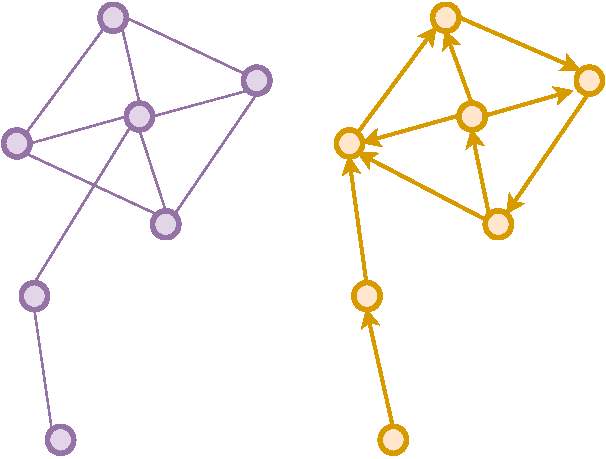
\includegraphics[scale = 0.8]{images/marcoteorico_graphdigraph.pdf}
    \caption{Ejemplos de una red dirigida y no dirigida. De lado izquierdo tenemos una red no dirigida. De lado derecho, una red dirigida. }
    \label{fig:marcoteorico_graph_digraph}
\end{figure}

\subsection{Red Multicapa y Red Temporal} 

Una característica compartida entre una red dirigida y una no dirigida es la \textit{propiedad estática} de los nodos y enlaces: La definición de los nodos y enlaces no es mutable [\cite{McGlohon2011}]. En consecuencia, este tipo de modelación tiene una limitación ante cambios del sistema. 


Indexar los nodos y aristas con una secuencia definida permite recuperar la mutabilidad del sistema. Cada uno de estos índices se define para representar los múltiples niveles o cambios del sistema. 
Una \textit{capa} ($L_{t}$) es una tupla de conjuntos de nodos y aristas

\begin{align*}
     & L_{t} = G_{t} (V_{t}, E_{t}),\\
    \text{donde } & E_{t} \subseteq E \text{ y }
    V_{t} \subseteq V ,\\
\end{align*}
donde $t$ es un índice para la capa $L_{t}$. Cabe mencionar que una capa puede ser vista como una sola red. Así, una \textit{red multicapa} es la sucesión de capas $\{L_{t}\}_{1}^{n}$, donde $n$ es el número de capas.

Un caso particular de las redes de multicapa es indexar el parámetro $t$ a un intervalo de tiempo. Este tipo de red es una red temporal.

Una \textit{red temporal} es una red multicapa donde el índice de las capas está asociado a un intervalo de tiempo. Este tipo de red permite una propuesta para describir la mutabilidad de una red a través del tiempo.  Es decir, esta red captura los cambios entre los  nodos y enlaces en periodos de tiempo definidos, a través de redes más simples. En la Figura \ref{fig:marcoteorico_redtemporal} se presenta un ejemplo de una red en distintos periodos de tiempo.


% Ejemplo de esto se puede ver en la figura \ref{fig:marcoteorico_redtemporal}, donde es una unión de redes no dirigidas. 

% En palabras generales, no es más que definir cada una de las redes con los nodos o enlaces de interés en el lapso de tiempo fijo. Definamos a $T$ como la longitud del lapso de tiempo. Por ejemplo, este valor de $T$ puede ser una hora o 25 minutos. 




\begin{figure}[h!]
    \centering
    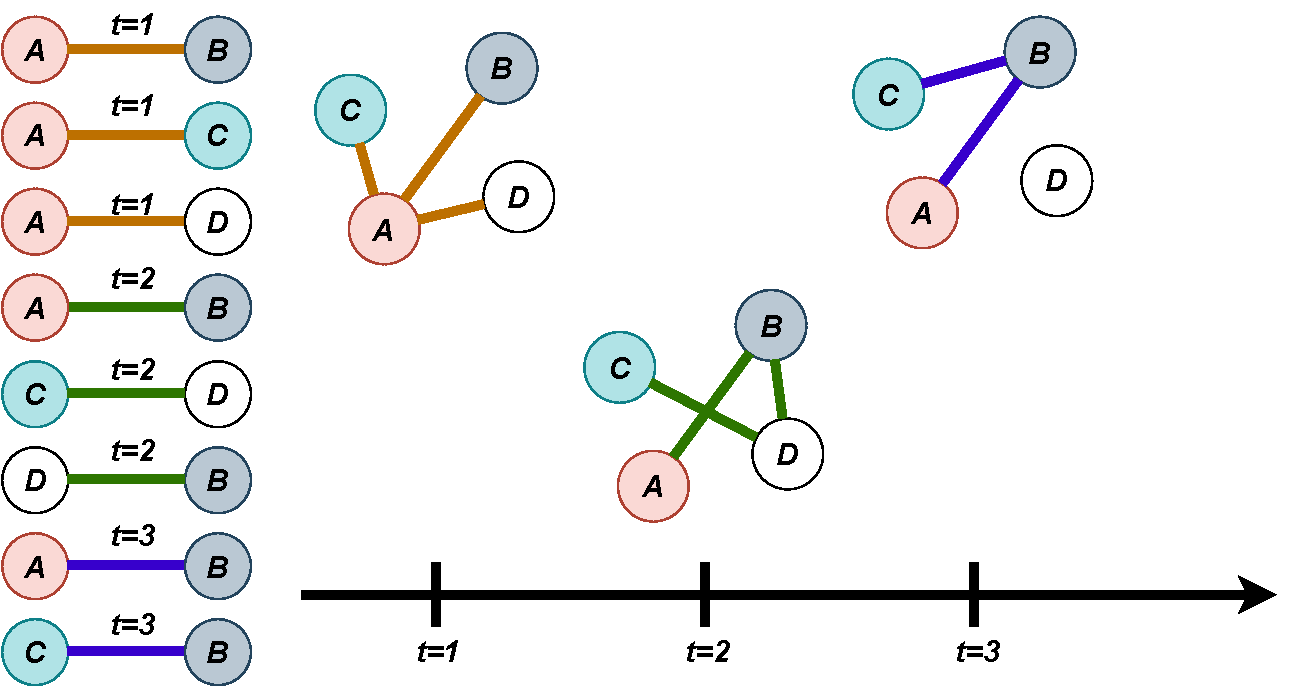
\includegraphics[scale = 0.6]{images/marcoteorico_redtemporal.drawio.pdf}
    \caption{Representación de una red temporal. Se observa como el enlace $(A,B)$ se mantuvo en cada periodo de tiempo. }
    \label{fig:marcoteorico_redtemporal}
\end{figure}

La extensión y definición de la red multicapa es extensa; puesto que permite añadir enlaces entre capas, entre nodos, etcétera. Este trabajo se basó en la red multicapa para definir la Red de la Dinámica Total (véase la sección 3.1).

Para mayor información sobre la red multicapa, se puede consultar [\cite{10.1093/comnet/cnu016}]

%-------------------------------------------------------------------------
%----------------------------------MÉTRICAS----------------------------------
%-------------------------------------------------------------------------
\subsection{ Métricas}


En esta sección, se presentan diversas métricas aplicadas en esta tesis. 




\subsubsection{Coeficiente de agrupamiento local (\textit{clustering}) }

Uno de los primeros patrones que hay en las redes es la aparición de \textit{ciclos}. Un ciclo es una \textit{trayectoria cerrada}; es decir, el nodo de inicio del camino es el mismo que el nodo final. 

% La \textit{longitud del camino} es el número de enlaces que contiene.
 El interés en la métrica nace por la medición de agrupación de nodos por sus enlaces [\cite{newman2018networks}]. El ciclo de longitud tres es de particular importancia  en el estudio de redes sociales, debido a que permite cuantificar la densidad local; es decir, la conexión de un nodo con los vecinos más cercanos  [\cite{kadushin2012understanding}].
 
% Densidad local ? 

 
%  Debido a que ayuda encontrar integración en el sistema social
 
%  En particular, el ciclo de longitud tres o \textit{triángulo}. 
 
%  El ciclo más interesante es el \textit{triángulo}. Un triángulo es un ciclo de longitud tres. 
 
 El coeficiente de agrupamiento es el conteo de aquellos triángulos existentes en la red sobre los triángulos que puedan existir. 
 
 

De manera formal, se fija a un nodo $v$. Se define $t_{v}$ como el número de triángulos donde el nodo $v$ es parte de éste y $d_{v}$ es el grado del nodo. Entonces, el coeficiente de agrupamiento ($C_{v}$) es: 

\begin{equation}
    \label{marcoteorico_clustering}
    C_{v} = \frac{ t_{v} }{ \frac{d_{v} (d_{v} - 1 )}{ 2 }} = \frac{2 t_{v} }{d_{v} (d_{v} - 1 ) }.
\end{equation}

El denominador de la expresión después del primer símbolo igual es el número de triángulos posibles entre sus vecinos. De la propia definición de la ecuación \ref{marcoteorico_clustering}, esta es no negativa y el valor máximo es uno. 


\subsubsection{Valor $k-\text{núcleo}$ (\textit{k-core}) }

La obtención de este valor se basa en la agrupación de nodos por su grado.

En palabras generales, este valor se obtiene al considerar el valor de $k$ más grande en los \textit{$k-core$} 
donde un nodo pertenece. Un $k-core$ de una gráfica es una subgráfica donde todos los nodos tienen un grado mayor o igual que  $k$.

De manera formal, el k-core $D_i$ está definido como 

\begin{equation}
    \label{marcoteorico_k-core_d_i}
    D_{i} = \{ v \in V | k_v \geq i \},
\end{equation}

Entonces, para un nodo $u \in V$, tenemos que su valor k-core es

\begin{equation}
    \label{marcoteorico_k-core_general}
    k-core(u) = \max \left\{ k \quad | \quad v \in D_k \right\}
\end{equation}

Como una consecuencia de la definición, se puede ver a $V = \bigcup_{i=1}^{k} D_i $. Esto último permite una visualización de la red en forma de capas con en la Figura \ref{fig:marco_teorico_kcore}.


% En este trabajo se consideró para cada nodo el valor máximo de $k$.

\begin{figure}[h!]
    \centering
    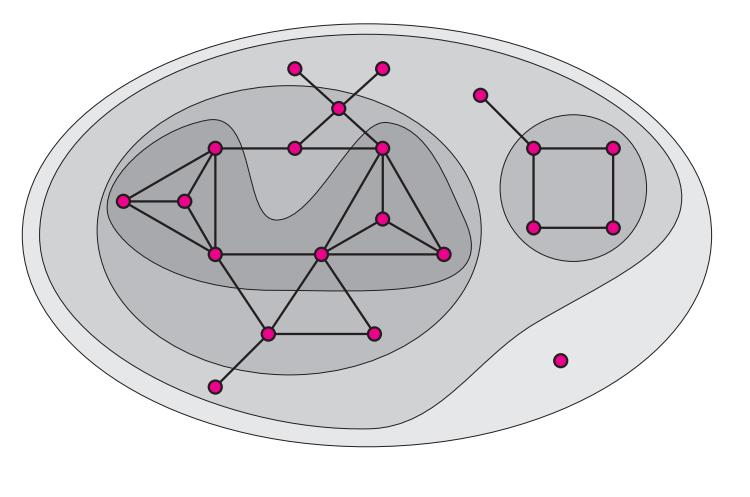
\includegraphics[scale = 0.5]{images/marcoteorico_kcore.png}
    \caption{Ejemplo visual de la aplicación de la métrica $k-\text{núcleo}$.
    (Fuente:  [\cite{DBLP:journals/corr/cs-DS-0310049}])}
    \label{fig:marco_teorico_kcore}
\end{figure}


\subsubsection{Métricas de Centralidad} 

El uso de las métricas de centralidad, para el enfoque social, tiene como objetivo identificar los nodos más importantes del sistema.
 
\subsubsection{Centralidad intermedia  (\textit{betweenness}) }

Es de suma importancia considerar los múltiples caminos que puede existir entre dos nodos.  En particular, aquellos caminos donde los nodos partícipes juegan un papel relevante en la red: los caminos más cortos. 

De manera formal, esta métrica se define como: 

\begin{equation}
    \label{eq:betweennes}
    B(v) = \sum_{v \neq j, i \in V} \frac{ \sigma( i,j | v) }{\sigma( i,j)} ,  
\end{equation}
donde $v \in V$, $\sigma(i,j)$ representa el número de caminos más cortos entre los nodos $i$ y $j$; y $\sigma(i,j|v)$ representa el número de caminos más cortos entre los nodos  entre $i$ y $j$ que pasan por el nodo $v$. 

La interpretación de esta métrica varía del objeto de estudio en cuestión. Sin embargo, en general, su interpretación denota la  importancia de algún nodo en la comunicación con los demás nodos en la red [\cite{newman2018networks}]. 


\subsubsection{Grado de cercanía (\textit{closeness}) }

Es el coeficiente de cercanía de un nodo hacia los demás nodos. Esta métrica pondera la suma de las distancias de un nodo fijo contra los demás nodos de la red y de este valor se obtiene su recíproco. Así, un valor alto en la suma de las distancias simboliza un grado bajo y, entonces, una importancia menor. 

De manera formal, si $d(u,v)$ representa la longitud del camino más corto entre $u$ y $v$: y $n$ es la cardinalidad del conjunto $V$. Entonces, el grado de cercanía de un nodo $u$ es 

\begin{equation}
    \label{marcoteorico_closeness}
    close(u) = \left(\frac{\sum_{v \neq u} d(u,v) }{n-1} \right) ^{-1}.
\end{equation}





\subsubsection{Centralidad de vector propio (\textit{eigenvector}) }


La noción de esta centralidad es medir la importancia de un nodo por la importancia de sus nodos vecinos. 

El cálculo de la misma es resolver una operación matricial: 

\begin{equation}
    \label{marcoteorico_eigenvector}
    A x = \lambda x,
\end{equation}
donde $A$ es la \textit{matriz de adyacencia} de la red y $\lambda > 0 $ es el valor propio más grande de la matriz de adyacencia.  

\subsubsection{Índice de Katz }

Una problemática con la expresión en la ecuación \eqref{marcoteorico_eigenvector} es que sólo involucra a los vecinos en la primera \textit{vecindad} de cada nodo. La n-ésima vecindad de un nodo se define como el conjunto de nodos donde hay un camino de longitud $n$. 

El índice de Katz extiende la noción de la influencia de nodos que pertenencen más allá de la primera vecindad. En efecto, el cálculo de la misma pondera su importancia a partir de todos los posibles caminos de longitud $k$ entre los nodos. 

\begin{equation}
    \label{marcoteorico_katz}
    Katz(i) &= \left[ \sum_{k = 0}^{\infty} ( \alpha A )^{k} e\right]_{ i }, 
\end{equation}
donde $e$ es el vector que en todas las entradas tiene el valor 1. La implementación de considerar todos los caminos de longitud $k$ está llevada a cabo por el producto matricial $A^{k}$. Nótese que, como en la métrica de vector propio, la ponderación es lineal debido a la definición de producto matricial. 




\begin{figure}[h!]
    \centering
    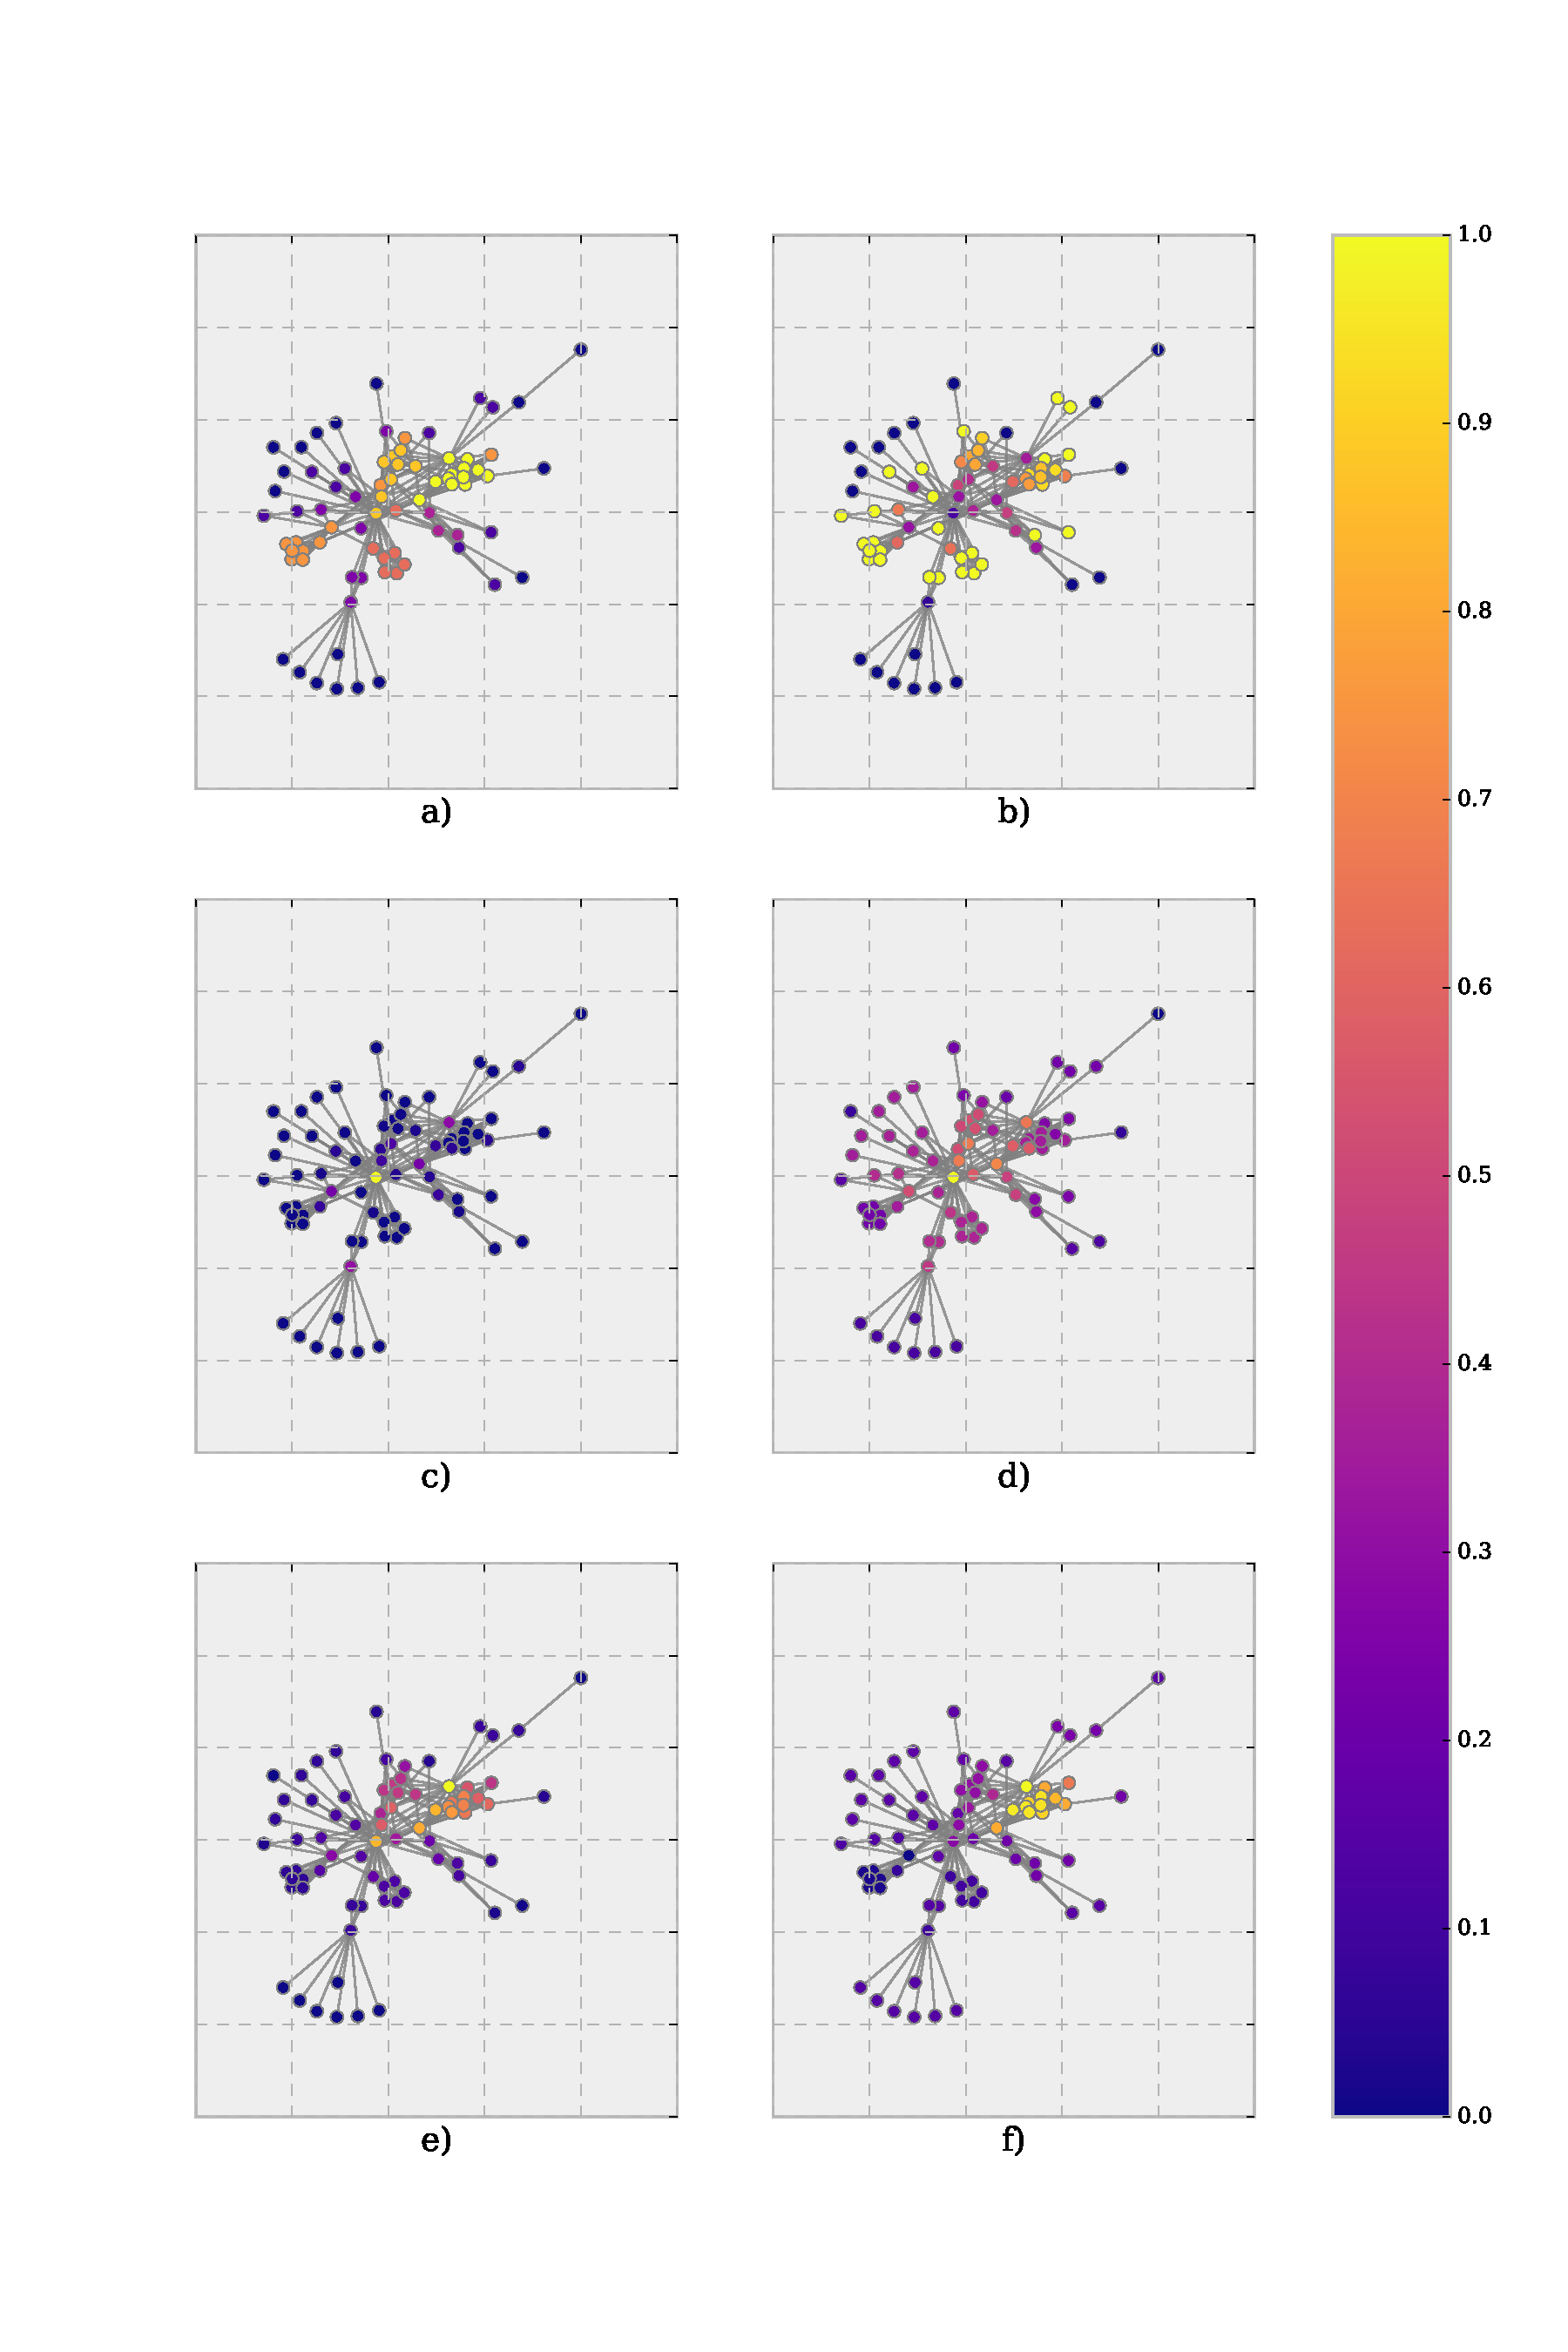
\includegraphics[scale = 0.40]{images/marcoteorico_barabasi (1).pdf}
    \caption{Comparativo de métricas para la red del Karate Club  de Zachary [\cite{Zachary_1977}]. Las métricas que se muestran son a) k-núcleo, b) clustering, c) betweeness, d) closeness, e) eigenvector y  f) centralidad de Katz.   Fuente: Elaboración propia.}
    \label{fig:marcoteorico_scale_free}
\end{figure}


%-------------------------------------------------------------------------
%----------------------Sistemascomplejos----------------------------------
%-------------------------------------------------------------------------
\newpage
\section{Sistemas Complejos.}

% Los sistemas complejos es el estudio de los sistemas estudian la forma de los componentes y su interacción entre sí.
Manlio de Domenico y Hiroki Sayama, en Complexity Explained [\cite{complejidad_explicada}], mencionan que los sistemas complejos   pueden espontáneamente auto-organizarse y presentar
estructuras globales y comportamientos no-triviales a mayores
escalas, sin intervención externa, autoridad central o líderes que
determinen el comportamiento colectivo [\cite{complejidad_explicada}]. 

Cabe mencionar que no es posible hablar de una definición formal de los sistemas complejos, sin embargo,  sí es posible identificar ciertas características, que a continuación se explican [\cite{Boulton2015-rb}].

\textbf{1. \textit{Sistémica} y \textit{sinérgica}}. La propiedad sistémica indica que es necesario explorar las relaciones o interconexiones de un sistema a fin de buscar patrones en las conexiones, sin embargo, dichas relaciones pueden ser lineales. En cambio, si las interacciones son no lineales entre las partes de un sistema, entonces se habla de la propiedad sinérgica.

\textbf{2. \textit{Multi escala.}}
Esta propiedad indica que para estudiar o entender un sistema es necesario considerar las diferentes escalas, incluyendo el tiempo, que forman parte del sistema. Además, las características que se presentan en una escala no deben asumirse en las demás, es decir, el estudio de una escala no permite entender el comportamiento de las demás escalas, lo cual indica que no debe considerarse \textit{auto similaridad}. 

\textbf{3. \textit{Resiliencia y adaptabilidad}}


La resiliencia de un sistema indica la capacidad que dicho sistema tiene para responder a variaciones internas y externas. Para el estudio de la resiliencia y la adaptación es necesario precisar dos conceptos:  \textit{variación}, que hace referencia a un cambio discreto a nivel individual; y,  \textit{fluctuación}, que hace referencia a un cambio en el fenómeno, como por ejemplo la densidad poblacional. Ahora bien, cuando las variaciones son entre los agentes de una misma especie de un sistema se conocen como \textit{microdiversidad}; mientras que variaciones de especies entre los agentes son conocidas como \textit{macrodiversidad}. 




\textbf{4. \textit{Incertidumbre.} } %Mi concepto de contingencia cambia
El futuro de un sistema es incierto, es decir, la secuencia o el orden de los eventos y el contexto en que se presentan son necesarios para determinar qué podría ocurrir.

%y ???(situación)  de este. 



\textbf{5. \textit{Autorregulación, auto-organización y emergencia.} }


%%

Estas propiedades están relacionadas con el estado del sistema y cómo cambios, tanto a  pequeña como a gran escala, afectan el estado del sistema final.

La propiedad de autorregulación permite al sistema fluctuar en un umbral de estabilidad; es decir, oscilar algunos valores cuantitativos sin cambiar  estados cualitativos.
La propiedad de  auto-organización permite al sistema modificar su estructura con base en interacciones locales. 

La propiedad de emergencia evoca un cambio radical y cualitativamente diferente partiendo del estado inicial. Este permite al sistema cambiar en su estructura permitiendo una nueva ramificación de estados y, por tanto, forzando la aparición de nuevos patrones de comportamiento.  
Las tres propiedades se basan en el mismo proceso, variaciones microscópicas que permiten cambios macroscópicos no lineales.


\newline

\subsection{Entropía}



La entropía es una medida formal de incertidumbre. El valor obtenido permite determinar tanto el nivel de incertidumbre como la información mostrada. Es decir, los sistemas que presentan un valor de entropía baja, indican que tienen baja incertidumbre y proporcionan poca información, por el contrario, cuando el sistema tiene un valor alto, indica mayor incertidumbre y mayor información revelada [\cite{cochardt2019scott}].





\subsubsection{Entropía de Shannon}

%La entropía de Shannon nos dice cuan eficiente es el flujo de información codificada.

%En teoría de la información se estudia como la información es afectada al codificarla en un sistema de transmisión. De forma ocasional, este estudio se  considera un subconjunto de la teoría de la comunicación [\cite{cover2006elements}].

%De esta forma, nacen métricas con una intuición sencilla pero aplicaciones complejas. 

Claude Shannon publicó en 1948 un artículo titulado \textit{A Mathematical Theory of Communication}, con el cual transformó el entendimiento de la información, al hacerla una cantidad bien definida y medible [\cite{stone2015information}].

La teoría de la información de Shannon proporciona una definición matemática de información, además, indica cuánta información se obtiene entre las diferentes partes o componentes de un sistema.

Entonces, la entropía se define como un promedio de la incertidumbre del verdadero estado de un fenómeno. Esto es, para una variable aleatoria $X$, con función de distribución de probabilidad $f(x)$, la entropía de Shannon se define como: 

\begin{equation}
    \label{shannon-entropy}
    H(X) = - \sum_{x} f(x) \log_{2} ( p(x)).
\end{equation}
El valor resultante, para el caso de $\log_{2}$, se llama $bits$ de información. 

La interpretación de esta métrica es sencilla, por ejemplo: ¿Cuántas preguntas con respuestas binarias se necesitan para saber el estado actual del sistema? Pues, entre mayor número de preguntas se necesiten mayor es la incertidumbre. Por el contrario, cuando $X$ tiene un sesgo para ciertos valores, la entropía es baja; ya que, el valor de $X$ es más probable que esté en la parte sesgada. 

Cabe mencionar que, se puede cambiar la base del logaritmo en esta métrica, obteniendo posibles resultados distintos (véase [\cite{cover2006elements}] para algunas propiedades). En este trabajo, por convención, únicamente se usará la entropía de Shannon con logaritmo en base 2.




\end{document}